%\begin{frame}[fragile]
%\frametitle{Designing MKM Formats}
%\begin{block}{Goals}
% \begin{itemize}
% \item expressive %, flexible 
%  \lec{ease of modeling}
% \item foundationally unconstrained 
%  \lec{coverage}
% \item minimal%Regular, 
%  \lec{ease of implementation}
% \item modular 
%  \lec{scalability}
% \item web-oriented
%  \lec{interoperability}
% \item $\ldots$
%\end{itemize}
%\end{block}
%
%\begin{block}{One key method: Extensibility}
%%\begin{itemize}
%%\item 
%%\end{itemize}
%\vs3em}
%\end{block}
%\end{frame}

\begin{frame}[fragile]
\frametitle{Designing MKM Formats}
\begin{block}{A design challenge}
\vspace{-1.5em}
\center{``Ease of modeling''\hspace{2em} vs \hspace{2em}``ease of implementation''}
\end{block}
\pause
\vspace{-1.5em}
\begin{columns}[t]
\column{4cm}
\begin{block}{Mathematics style}
\begin{lstlisting}
<theorem name="foo">
   $1 + 1\doteq 2$
</theorem>

<proof for="foo">
   $proof\textrm{-}term$
</proof>
\end{lstlisting}
\vspace{.85em}
\end{block}
\column{4cm}
\begin{block}{Curry-Howard style}
\begin{lstlisting}
<constant name="foo">
  <type>
    $1 + 1\doteq 2$
  </type>
  <definition>
     $proof\textrm{-}term$
  </definition>
</constant>
\end{lstlisting}
\end{block}
\end{columns}
\pause
\begin{block}{Standard solution: \alert{Extensibility}}
\vspace{-.3em}
Minimal core + extension principles %(macros, notations etc.)
\end{block}
\end{frame}


\begin{frame}[fragile]
\frametitle{Classification of Extension Principles}%Extensibility}
\begin{block}{What does the extension principle introduce?}
\vspace{-.5em}
\begin{itemize}
\item new object (typically identifier)
\lec{e.g., $2 := succ(succ(zero))$}%\texttt{{\backslash}newcommand\{{\backslash}mycom\}\{...\}}}
\item new statement (typically with keyword)
\lec{e.g., locales in Isabelle} %case-based function definitions %e.g., \verb+\newenvironment{\myenv}{...}{...}+}
\end{itemize}
\end{block}

\begin{block}{Who defines the extension principle?}
\vspace{-.5em}
 \begin{itemize}
 \item the user 
 \lec{e.g., $2 := succ(succ(zero))$}
 \item the programmer
 \lec{e.g., locales in Isabelle}
 \end{itemize}
\end{block}

\begin{block}{How is the extension principle interpreted?}
\vspace{-.5em}
 \begin{itemize}
 \item unconstrained
 \lec{interpretation at runtime}
 \item constrained
 \lec{well-formedness judgments}% validate extension}
 \end{itemize}
\end{block}

%\begin{block}{What does an extension introduce?}
%\vspace{-.3em}
%\alert{object vs statement}%\\\pause
%%E.g., Introduce new symbols via notations vs new declarations via definitions
%\end{block}
%\begin{itemize}
%\item E.g., LaTeX macros \verb+\newcommand{\mycommand}{...}+, \verb+\newenvironment{\myenv}{...}{...}+
%\end{itemize}
%\pause
%\begin{block}{Who can introduce an extension?}
%\vspace{-.3em}
%\alert{user vs developer}
%\end{block}
%\pause
%\begin{block}{How is an extension evaluated?}
%\vspace{-.3em}
%\alert{unconstrained vs constrained}
%\end{block}
\end{frame}

%\begin{frame}[fragile]
%\frametitle{}
%\begin{columns}
%\column{5cm}
%\begin{lstlisting}
%<theory name="foo">
%   1 + 1 = 2
%</theory>
%
%<proof for="foo">
%   $\ded\ldots$
%</proof>
%\end{lstlisting}
%
%\column{5cm}
%\begin{lstlisting}
%<constant name="foo">
%  <type>
%    1 + 1 = 2
%  </type>
%
%  <definition>
%     $\ded\ldots$
%  </definition>
%</constant>
%\end{lstlisting}
%\end{columns}
%\end{frame}


%\begin{frame}[fragile]
%\frametitle{}
%\begin{multicols}{2}
%\begin{lstlisting}%[mathescape]
%<theorem name="foo">
%  1 + 1 = 2
%</theory>
%
%<proof for="foo">
% $\proof\ldots$
%</proof>
%\end{lstlisting}
%
%\begin{lstlisting}%[mathescape]
%<constant name="foo">
% <type>
%  1 + 1 = 2
% </type>
% <definition>
% ``proof term''
% </definition>
%</constant>
%\end{lstlisting}
%\end{multicols}
%\end{frame}

%\begin{frame}
%\begin{tabular}{ll}
%\only<1>{A & B} \\
%\only<2>{C & D}
%\end{frame}

\begin{frame}
\frametitle{Some Extensible MKM Formats}
\begin{center}
\begin{tabular}{c|l|c|c|}
\multicolumn{2}{c}{} & \multicolumn{2}{c}{Extensions} \\
\cline{3-4}
\multicolumn{2}{c|}{} & Object Level & Statement Level \\
\cline{2-4}
\\[-.8em]
\cline{2-4}
\multirow{8}{*}{\begin{sideways} MKM Formats \end{sideways}} 
& LaTeX & \user & \user  \\
\cline{3-4}
& (narrative) & \unconst & \unconst\\
\cline{2-4}
\\[-.8em] 
\cline{2-4}
& Isabelle/HOL & \user & \prog \\
\cline{3-4}
& (formal math) & \un\const & \unconst\\
\cline{2-4}
\\[-.8em] 
\cline{2-4}
& OMDoc 1.2 & \user & \prog \\
\cline{3-4}
& (content markup) & \const & \unconst\\
\cline{2-4}
\end{tabular}
\end{center}
\pause
\begin{block}{LaTeX}
\begin{itemize}
\item Object level: e.g., $\mathtt{\backslash{newcommand}\{\backslash{mycommand}\}\{\ldots\}}$
\item Statement level: e.g., $\mathtt{\backslash{newenvironment}\{\backslash{myenv}\}\{\ldots\}\{\ldots\}}$
\end{itemize}
\end{block} 
\end{frame}

\begin{frame}
\frametitle{Some Extensible MKM Formats}
\begin{center}
\begin{tabular}{c|l|c|c|}
\multicolumn{2}{c}{} & \multicolumn{2}{c}{Extensions} \\
\cline{3-4}
\multicolumn{2}{c|}{} & Object Level & Statement Level \\
\cline{2-4}
\\[-.8em]
\cline{2-4}
\multirow{8}{*}{\begin{sideways} MKM Formats \end{sideways}} 
& LaTeX & \user & \user  \\
\cline{3-4}
& (narrative) & \unconst & \unconst\\
\cline{2-4}
\\[-.8em] 
\cline{2-4}
& Isabelle/HOL & \user & \prog \\
\cline{3-4}
& (formal math) & \un\const & \unconst\\
\cline{2-4}
\\[-.8em] 
\cline{2-4}
& OMDoc 1.2 & \user & \prog \\
\cline{3-4}
& (content markup) & \const & \unconst\\
\cline{2-4}
\end{tabular}
\end{center}
\only<1>{
\begin{block}{Isabelle/HOL}
\vspace{-.2em}
\begin{itemize}
\item Object level: definitions, declarations, etc.
\item Statement level: locales, type defns, case-based function defns
\end{itemize}
\end{block}
}
\only<2>{
\begin{block}{OMDoc 1.2}
\begin{itemize}
\item Object level: symbol declarations
\item Statement level: theorems, definitions, proofs, etc.
\end{itemize}
\end{block}
}
\end{frame}

\begin{frame}
\frametitle{Our Approach: Generic Framework for Extension Principles}
\only<1>{
\begin{center}
\begin{tabular}{c|l|c|c|}
\multicolumn{2}{c}{} & \multicolumn{2}{c}{Extensions} \\
\cline{3-4}
\multicolumn{2}{c|}{} & Object Level & Statement Level \\
\cline{2-4}
\\[-.8em]
\cline{2-4}
\multirow{8}{*}{\begin{sideways} MKM Formats \end{sideways}} 
& LaTeX & \user  & \user\\
\cline{3-4}
& (narrative) & \unconst & \unconst\\
\cline{2-4}
\\[-.8em] 
\cline{2-4}
& Isabelle/HOL & \user & \prog \\
\cline{3-4}
& (formal math) & \un\const & \unconst\\
\cline{2-4}
\\[-.8em] 
\cline{2-4}
& OMDoc 1.2 & \user & \prog \\
\cline{3-4}
& (content markup) & \const & \unconst\\
\cline{2-4}
\\[-.8em]
\cline{2-4}
& \multirow{2}{*}{\alert{Our approach}} & \user & \user \\
\cline{3-4}
&  & \const & \const\\
\cline{2-4}
\end{tabular}
\end{center}
%\center{\alert{A generic framework for arbitrary extension principles}}
}
\only<2>{
\begin{center}
\begin{tabular}{c|l|c|c|}
\multicolumn{2}{c}{} & \multicolumn{2}{c}{Extensions} \\
\cline{3-4}
\multicolumn{2}{c|}{} & Object Level & Statement Level \\
\cline{2-4}
\\[-.8em]
\cline{2-4}
& OMDoc 1.2 & \user & \prog \\
\cline{3-4}
& (content markup) & \const & \unconst\\
\cline{2-4}
\\[-.8em]
\cline{2-4}
& \alert{OMDoc 2} & \user & \user \\
\cline{3-4}
& \alert{(content markup)} & \const & \const\\
\cline{2-4}
\end{tabular}
\end{center}
\vspace{.5em}
\begin{block}{Redesign the OMDoc format}%via our generic extension framework}
\vspace{-.3em}
\begin{center}
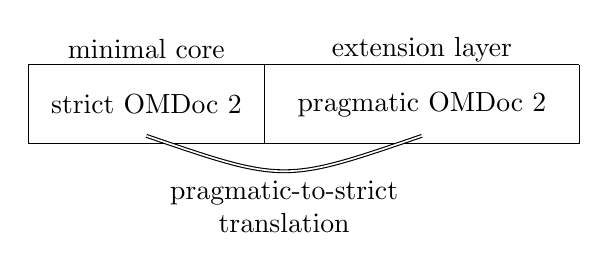
\begin{tikzpicture}
\draw[-] (0,1) -- (3,1);
\draw[-] (0,0) -- (3,0);
\draw[-] (0,1) -- (0,0);
\draw[-] (3,1) -- (3,0);
\node(s) at (1.5,.5) {\alert{strict OMDoc 2}};
\node(m) at (1.5,1.2) {minimal core};

\draw[-] (3,0) -- (7,0);
\draw[-] (3,0) -- (7,0);
\draw[-] (3,1) -- (7,1);
\draw[-] (7,1) -- (7,0);

\node(p) at (5,.5) {\alert{pragmatic OMDoc 2}};
\node(e) at (5,1.2) {extension layer};

\draw[double,-\arrowtip] (5,.1) .. controls (3.25,-.5) .. node[below] {\alert{pragmatic-to-strict}} (1.5,.1);
\node at (3.25,-1) {\alert{translation}};
\end{tikzpicture}
\end{center}
\vspace{-.5em}
\end{block}
}
\end{frame}

\begin{frame}
\frametitle{Motivating Example}
%\only<3>{
%\begin{center}
%\end{center}

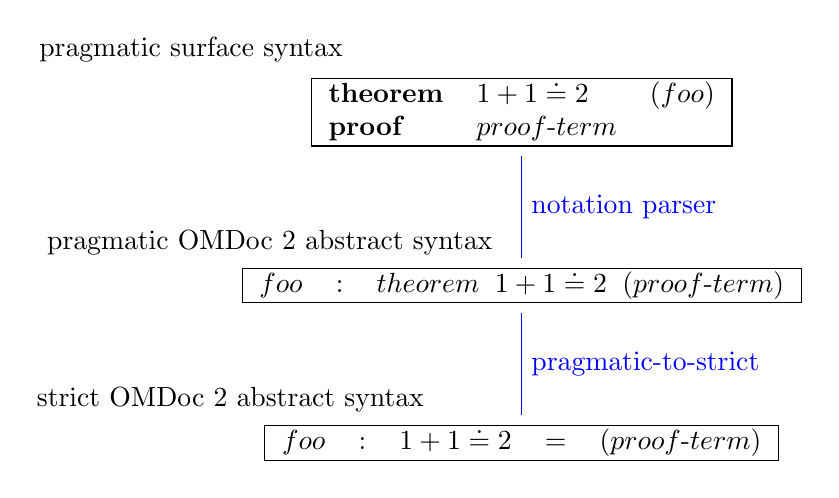
\begin{tikzpicture}
\node(n) at (4,4.2) {
\begin{tabular}{|lll|}\hline
\textbf{theorem} & $1 + 1 \doteq 2$ & $(foo)$ \\
\textbf{proof}   & $proof\textrm{-}term$ &\\
\hline
\end{tabular}
};

\node at (-.2,5) {\alert{pragmatic surface syntax}};
\node at (.8,2.55) {\alert{pragmatic OMDoc 2 abstract syntax}};
\node at (.3,.55) {\alert{strict OMDoc 2 abstract syntax}};
\node(p) at (4,2) {
\begin{tabular}{|lll|}\hline
$foo$ &:& $theorem\;\;1 + 1 \doteq 2\;\;(proof\textrm{-}term)$\\\hline
\end{tabular}
};

\node(s) at (4,0) {
\begin{tabular}{|lllll|}\hline
$foo$ &:& $1 + 1 \doteq 2$ &=& $(proof\textrm{-}term)$\\\hline
\end{tabular}
};

\draw[blue,-\arrowtip] (n) --node[right] {notation parser} (p);
\draw[blue,-\arrowtip] (p) --node[right] {pragmatic-to-strict} (s);
\end{tikzpicture}
%}
\end{frame}



%\begin{frame}
%\frametitle{}
%\begin{itemize}
% \begin{itemize}
% \item Languages for formalized math 
%  \lec{e.g. Isabelle}
% \item Narrative formats for math
%  \lec{e.g. TeX/LaTeX}
% \end{itemize}
%\item Language extensions for content markup formats
% \begin{itemize}
% \item Core language
%  \lec{e.g., strict content MathML}
% \item Extension
%  \lec{e.g., pragmatic content MathML}
% \item Translation
%  \lec{e.g., strict content MathML translation}
% \end{itemize}
%\item Twelf: defined/undefined constants $c : T = D$
%\item Isabelle: type definitions 
%\item Mizar: implicit, case-based definitions, 
%\item Coq: recursive case-based function definitions
%\end{itemize}
%\end{frame}


